\exercice Copilote
\begin{center}
%\fbox{
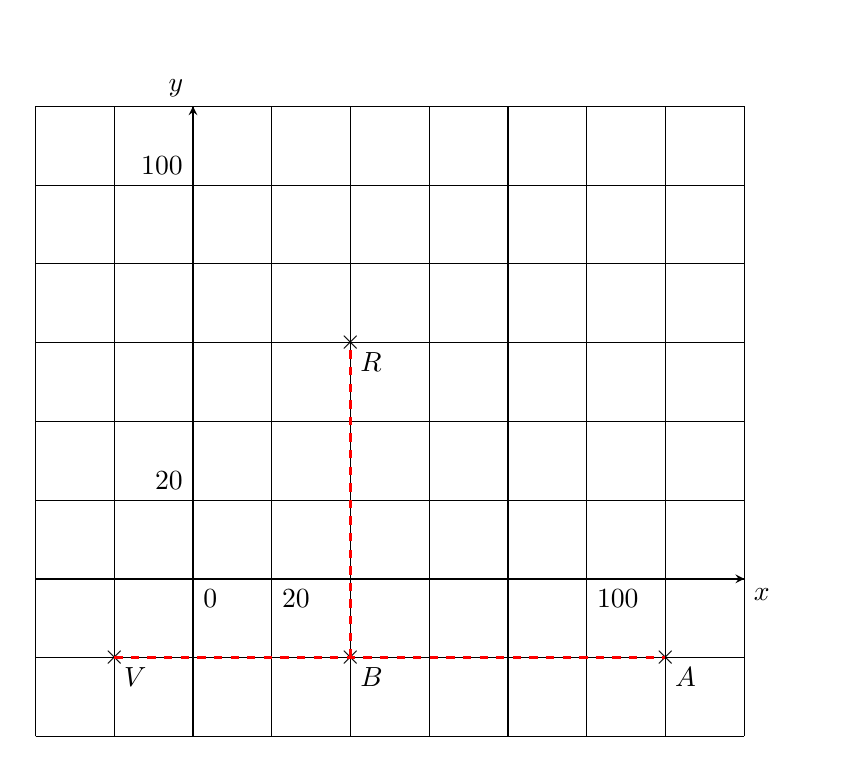
\begin{tikzpicture}[scale=1,every node/.style={scale=1}]
	%Points
	\clip (-2.1,-2.1) rectangle (8,7);
	\coordinate(O)at(0,0);
	\coordinate(I)at(1,0);
	\coordinate(J)at(0,1);
	\coordinate(xstart)at(-2,0);
	\coordinate(xend)at(7,0);
	\coordinate(ystart)at(0,-2);
	\coordinate(yend)at(0,6);
	\coordinate(V)at(-1,-1);
	\coordinate(B)at(2,-1);
	\coordinate(R)at(2,3);
	\coordinate(A)at(6,-1);
	%Étiquettes
%	\draw (I) node[below right] {$1$};
%	\draw (J) node[above left] {$1$};
	\draw (xend) node[below right] {$x$};
	\draw (yend) node[above left] {$y$};
	%%%%%%%%%%%%%%%%%%%%%%%%%%%%%%%%%%%%
	%Axes
	\draw [thick] (xstart) -- (xend);
	\draw [thick] (ystart) -- (yend);
	%Flèches
%	\draw [>=stealth,->] (O) -- (I);
%	\draw [>=stealth,->] (O) -- (J);
	\draw [>=stealth,->] (O) -- (xend);
	\draw [>=stealth,->] (O) -- (yend);
	%Grille
	\draw [thin] (-2,-2)grid(7,6);
	%%%%%%%%%%%%%%%%%%%%%%%%%%%%%%%%%%%%
	%étiquettes
	\foreach \point in {V,B,R,A}
		\draw(\point)node{$\times$};
	\foreach \point in {V,B,R,A}
		\draw(\point)node[below right]{$\point$};	
	
    	\draw[thick, below right] (0,0) node{0};
    	\draw[thick, below right] (1,0) node{20};
    	\draw[thick, below right] (5,0) node{100};
    	\draw[thick, above left] (0,1) node{20};
    	\draw[thick, above left] (0,5) node{100};
    
	\draw [thick,dashed,red] (V) -- (A);
	\draw [thick,dashed,red] (B) -- (R);
	
%		\only<6-|handout:5->{\draw [thick,red] (B) -- (R) node[midway,above,sloped] {$80$};}
%		\only<7-|handout:6->{\draw [thick,green] (V) -- (R) node[midway,above,sloped] {$100$};}
%		\only<4-4|handout:4->{\draw [thick,blue] (V) -- (5,-1) node[near end,below,sloped] {$120$};}
%		\only<4-6|handout:4-5>{\draw [thick,blue] (V) -- (R) node[midway,above,sloped] {$?$};}
%		\only<5-|handout:5->{\draw [thick,red] (V) -- (B) node[midway,below,sloped] {$60$};}
	
\end{tikzpicture}
%}
\\[2em]
\end{center}
À quelques kilomètres de l'arrivée d'une course automobile, le véhicule situé en $V$ doit prendre une décision~:\\	
Peut-il tenter d'aller jusqu'à l'arrivée~$A$ directement ou bien doit-il passer par le ravitaillement~$R$~? Votre rôle de copilote est de l'aider à prendre cette décision.\\ Que lui conseillez-vous ?\\ \textcolor{red}{Il lui reste 120km d'autonomie.}\\
Les points $V$, $R$ et $A$ placés dans le repère orthonormé représentent respectivement les positions de la voiture, du ravitaillement et de l'arrivée.
\vspace{-2em}	
